% !TEX root = ./Vorlesungsmitschrift DIFF 2.tex  
\lecture{Do 16.07. 10:15}{}
\begin{definition}
  Sei \( U\subset\reals^m \) offen (\( n \)-dimensionale Untermannigfaltigkeit des \( \reals^m \)).
  Ein \define{Tensorfeld} auf \( U \) (\( s \)-fach kontravariant, \( r \)-fach kovariant) ist eine Abbildung
  \begin{equation*}
      \alpha\maps U\ni a \mapsto \alpha(a)\in \tensors{r}{s}{\tangentialraum{a}{U}}.
  \end{equation*}
  Eine \define{Differentialform} von Grad \( r \) ist eine Abbildung
  \begin{equation*}
      \omega\maps U\ni a \mapsto \omega(a)\in\exterior+{r}{\tangentialraum{a}{\dualspace{U}}}
  \end{equation*}
  \( \differentialforms{r}{U}=\set{\omega \text{ Differentialform vom Grad \( r \)}} \).
  \( \alpha \) wird \( \stetigefunktionen[k] \) genannt, falls 
  \begin{equation*}
      U\ni a \mapsto \alpha(a)(u_1,\dotsc ,u_r,w^1,\dotsc ,w^s)\in\reals
  \end{equation*}
  für jedes fest gewählte Tupel 
  \begin{equation*}
      (u_1,\dotsc ,u_r,w^1,\dotsc ,w^s)\in (\tangentialraum{a}{U})^r\times (\tangentialraum{a}{\dualspace{U}})^s
  \end{equation*}
  \( \stetigefunktionen[k] \) ist.

  Speziell ist \( \omega\in\Omega(U) \) \( \stetigefunktionen[k] \) falls 
  \begin{equation*}
      U\ni a \mapsto \omega(a)(u_1,\dotsc ,u_r)\in\reals
  \end{equation*}
  \( \stetigefunktionen[k] \) ist für jedes \( (u_1,\dotsc ,u_r)\in(\tangentialraum{a}{U})^r \).
\end{definition}

\begin{bemerkung*}
  \begin{enumerate}
      \item Tensorfelder und Differentialformen vom Grad 0 sind Funktionen 
      \item Ein einfach kontravariantes Tensorfeld ist ein Vektorfeld:
      \(\alpha(a)\in \covarianttensors{1}{\tangentialraum{a}{\dualspace{U}}}\)
      \begin{gather*}
          \alpha(a)\in(\tangentialraum{a}{\dualspace{U}})^*\approx \tangentialraum{a}{U},\\
          \alpha(a)=\sum_{i=1}^{m}\alpha(a)^i e_i
      \end{gather*}
      mit \( (e_1,\dotsc ,e_n) \) eine Basis von \( \tangentialraum{a}{U} \).
  \end{enumerate}
\end{bemerkung*}

\begin{blank*}[Koordinatendarstellung]
  Sei \( \varphi\maps U\to\reals^m \) die kanonische Parametrisierung von \( U \), \( \varphi(x)=x \).
  Dann ist (\vgl \ref{tangentialraum_durch_parametisierung})
  \begin{equation*}
      \tangentialraum{x}{U}=\Span{\explain{\text{kanonische Einheits-Basis}}{e_1,\dotsc ,e_m}}
  \end{equation*}
  Die dazu duale Basis bezeichnet man mit \( \differential x^1,\dotsc ,\differential x^m \).
  Es gilt für \( v=\sum v^i e_i\in \tangentialraum{x}{U} \):
  \begin{equation*}
      \differential x^j(v)=v^j.
  \end{equation*}
  Nach Bemerkung \ref{exterior_basis} nach \thref{wedge_product} ist 
  \begin{equation*}
      \Set{\differential x^{j_1}\wedge\dotsb \wedge \differential x^{j_r}| j_i\in\set{1,\dotsc ,n},j_1<j_2<\dotsb<j_r}
  \end{equation*}
  eine Basis von \( \differentialforms{r}{U} \), also 
  \begin{equation*}
      \omega\in\differentialforms{r}{U}\implies \omega=\sum_{\mathclap{j_1<\dotsb<j_r}} \omega_{j_1\cdots j_r}\differential x^{j_1} \wedge\dotsb \wedge \differential x^{j_r}
  \end{equation*}
  mit Funktionen \( \omega_{j_1\cdots j_r}\maps U\to\reals \).
  Beachte: \( \omega \) ist genau dann \( \stetigefunktionen[k] \) wenn \( \omega_{j_1\cdots j_r}\) \( \stetigefunktionen[k] \) ist.

  \begin{beispiel*}
      \( m=2\), \(u,v\in \tangentialraum{a}{U}\cong\reals^2 \)
      \begin{equation*}
          \differential x^1\wedge \differential x^2 (u,v)=\determinant{ 
          \begin{pNiceMatrix} \differential x^1(u) & \differential x^1(v)\\ \differential x^2(u) & \differential x^2(u) \end{pNiceMatrix} }
          =\determinant{
          \begin{pNiceMatrix} u^1 & v^1 \\ u^2 & v^2 \end{pNiceMatrix}}
      \end{equation*}
  \end{beispiel*}
\end{blank*}

\begin{definition} \label{pullback}
  Sei \( \varphi\maps U\to\reals^n\) \(\stetigefunktionen[1]\), \( U\subset\reals^m \) offen mit \( \varphi(U)=V \) offen.
  Sei \( \omega\in\differentialforms{r}{V} \). Dann definiert 
  \begin{gather*}
      \p*{ \diffpullback{\varphi} \omega }(t)(v_1,\dotsc ,v_r)\coloneqq \omega\p*{ \varphi(t) }
      \p*{ D\varphi(t)v_1,\dotsc ,D\varphi(t)v_r }\quad  \forall t\in U,\logicspace  \forall v_1,\dotsc ,v_r\in\reals^m
  \end{gather*}
  \( r \)-Form auf \( U \), \( \diffpullback{\varphi}{\omega}\in\differentialforms{r}{U} \), den sogenannten \define{pullback (Zurückziehung)}   von \( \omega \) unter \( \varphi \).

  In Koordinaten: 
  \begin{equation*}
      \omega=\sum_{\mathclap{i_1<\dotsb <i_r}} \omega_{i_1\cdots i_r}\differential x^{i_1}\wedge\dotsb \wedge \differential x^{i_k}.
  \end{equation*}
  Dann ist \( \diffpullback{\varphi}{\omega}=\sum \omega_{i_1\cdots i_r}\circ\varphi d\varphi^{i_1}\wedge\dotsb \wedge d\varphi^{i_k}  \) mit 
  \begin{equation}
      \tag{\( * \)} \label{eq:pullback}
      \differential\varphi^i=\sum_{k=1}^{m}\partial_k\varphi^i \differential{t^k}
  \end{equation}
  Beweis durch Nachrechnen. \( \diffpullback{\varphi}{\omega} \) ist also tatsächlich in \( \differentialforms{r}{U} \).
\end{definition}

\begin{definition}
  \define{Cartan-Ableitung} (äußere Ableitung) \( U\subset\reals^n \).
  \( f\in\differentialforms{0}{U} \) sei \( \stetigefunktionen[k] \) mit \( k\geq 1 \). Dann setze:
  \begin{equation*}
      \differential f \coloneqq \sum_{j=1}^{m}\partial_j f\differential x^j \quad (\text{Siehe oben \eqref{eq:pullback}})
  \end{equation*}
  \( \omega\in\differentialforms{r}{U} \) sei \( \stetigefunktionen[k] \) mit \( k\geq 1 \). Dann setze:
  \begin{equation*}
      \differential \omega\coloneqq \sum_{\mathclap{q \leq i_1<\dotsb <i_r \leq n}} \differential{(\omega_{i_1\dotsm i_r})}\wedge \differential x^{i_1}\wedge\dotsb \wedge \differential x^{i_r}
  \end{equation*}
  \( \differential \omega\in\differentialforms{r+1}{U} \)
\end{definition}

\begin{beispiel*}
  \( \omega=p\differential x+q\differential y \) 
  \begin{align*}
      \differential{\omega} &=  \p*{ \cancel{\partial_1p\differential x}+\partial_2p\differential y }\wedge \differential x
      +\p*{ \partial_1 q\differential x+\cancel{\partial_2 q\differential y} }\wedge \differential y\\
      &= \p*{ \partial_1 q-\partial_2 p }\differential x\wedge \differential y
  \end{align*}
  \( \differential{\omega}=0 \) falls \( \partial_1q=\partial_2p \) Integrabilitätsbedingung bei den \emph{exakten} DGLn

  Das ist insbesondere der Fall, wenn \( \omega=\differential{(f)}, f(x,y),\partial_1f=p,\partial_2f=q\quad f\in \stetigefunktionen[2] \).
  Beachten Sie die Ähnlichkeit zum \hyperref[integralsatz_gauss]{Satz von Gauß} in 2 Dimensionen \( \leadsto \) später mehr.
\end{beispiel*}

\begin{blank}
  \begin{bemerkung*}
    Teilweise längere Rechnungen zeigen: \( \omega,\tilde{\omega}\) \( \stetigefunktionen[k]\), \( k\geq 1. \)

    \begin{itemize}
      \item \( \differential\maps \differentialforms{r}{U}\to\differentialforms{r+1}{U} \) ist linear 

      \item \( \differential{(\omega\wedge\tilde{\omega})}=\differential{\omega\wedge\tilde{\omega}+(-1)^r\omega\wedge\tilde{\omega}} \) für \( \omega\in\differentialforms{r}{U} \)
  
      \item \( \differential{(\differential{\omega})}=0 \), \( \omega\) \( \stetigefunktionen[k]\), \( k\geq 2 \).
    \end{itemize}
  \end{bemerkung*}
  \begin{definition*}
    \( \omega\in\differentialforms{r}{U} \) heißt \emph{geschlossen} falls \( \differential{\omega}=0 \) und \emph{exakt} falls \( \exists \alpha\in\differentialforms{r-1}{U} \) \sd \( \differential{\alpha}=\omega \).
    \( \alpha \) heißt \define{Potential} für \( \omega \). \( U\subset\reals^m \)
    Ist \( \differential{\omega}=0 \), \( U \) sternförmig, \dh \texists Punkt \( a\in U \) \sd die Verbindungslinien von \( a \) zu allen Punkten von \( U \) in \( U \) liegen, so \texists Potential.
    Die Konstruktion funktioniert im wesentlichen so, wie bei den exakten DGLn (Partielle Integration entlang der Verbindungslinien).
    \emph{Lemma von Poincaré}
  \end{definition*}
\end{blank}
\begin{bemerkung}
  Zusammenhang zu Differentialgleichungen: 
  \begin{enumerate}
      \item Exakte DGLn: Schreibe statt \( g(x,y)y'+h(x,y)=0 \)
      \begin{equation*}
          \omega\coloneqq g(x,y)\differential{y}+h(x,y)\differential{x}.
      \end{equation*}
      Die Integrabilitätsbedingung impliziert \( \differential{\omega}=0 \) \timplies (auf sternförmigem Gebiet) \texists  \(  f \) \sd \( \omega=\differential{f} \) (also exakt), \( g=\partial_y f\), \( h=\partial_x f \),
      \hyperref[satz_von_der_impliziten_funktion]{Satz über implizite Funktionen}: \texists  \(  x \mapsto y(x)\) \sd \( f(x,y(x))=0\to  \) die Lösung \( y(x) \) der DGL.\@
      \item Merkregel bei DGLn mit getrennten Variablen. Schreibe statt \( y'=f(x)g(y) \)
      \begin{equation*}
          \frac{1}{g(y)} \differential{y}=f(x)\differential{x}
      \end{equation*}
  \end{enumerate}
\end{bemerkung}

\section{Zusammenhang zu Integration auf Untermannigfaltigkeiten}

\begin{definition}
  \( U\subset\reals^m \) offen, \( \omega=f\differential{x^1}\wedge\dotsb \wedge\differential{x^m} \).
  \( \omega \) heißt \emph{integrierbar} über \( V\subset U\) falls \(\evaluateat{f}{V} \) integrierbar ist.
  Man setzt dann:
  \begin{equation*}
      \int_V\omega\coloneqq \int_V f\differential{x^1}\wedge\dotsb \wedge\differential{x^m}\coloneqq \int_V f(x)\differential{x}
  \end{equation*}
\end{definition}

\begin{lemma}\label{uebertragung_integral}
  \( U,V\subset\reals^m \) offen, \( \varphi\maps U\to\reals^m\), \( \varphi(U)=V \), Diffeomorphismus auf \( V \).
  Sei \( K\subset U \) kompakt.
  Dann gilt 
  \begin{align*}
      \int_{\varphi(K)}\omega &=\hspace*{0.87em} \int_{K}\diffpullback{\varphi}{\omega}\quad \mathrm{falls }\determinant{\totalderivative{\varphi}}>0\\
      &= -\int_{K} \diffpullback{\varphi}{\omega} \quad \mathrm{falls }\determinant{\varphi}<0
  \end{align*}
\end{lemma}

\begin{proof}
  \( \omega=f\differential{x^1}\wedge\dotsb \wedge\differential{x^m} \) \timplies
  \( \diffpullback{\varphi}{\omega}=\p*{ f\circ\omega }\determinant{\differential{\varphi}}\differential{x^1}\wedge\dotsb \wedge\differential{x^m} \) (nachrechnen).
  Die Behauptung folgt mit der \hyperref[transformationssatz]{Transformationsformel}
  \begin{equation*}
      \int_{\varphi(K)}\omega=\int_{\varphi(K)}f\differential{x}=\int_{K}f\p*{ \varphi(y) }\abs{\determinant{\totalderivative{\varphi(y)}}}\differential{y}
  \end{equation*}
\end{proof}

Diese Definition können wir auf beliebige \define{orientierbare Untermannigfaltigkeiten} übertragen.
Orientierbar: \texists Beschreibung durch lokale Parametrisierungen 
\begin{equation*}
  \Set{\varphi\maps U_i\to V_i|i\in I}
\end{equation*}
\sd 
\begin{equation*}
  \Phi_{ij}\coloneqq \varphi^{-1}_i\circ\varphi_j\maps\varphi^{-1}(V_i\cap V_j)\to\varphi^{-1}(V_i\cap V_j)
\end{equation*}
\( \determinant{ \totalderivative{\Phi_{ij}}}>0 \) erfüllt.

Wählt man eine Basis \( \p*{ \partial_j\psi }_{j=1\cdots m} \) von \( \tangentialraum{a}{M} \) und ist \( a\in\varphi(U)\cap\psi(\tilde{U}) \) so ist \( \p*{\p*{ \partial_j\psi }_{j=1,\dotsc, m}  } \) gleich orientiert, \dh der Basiswechsel \( A \) hat positive Determinante:
\begin{equation*}
  \totalderivative{\varphi}=\big(\totalderivative{(\underbrace{\varphi^{-1}\circ\psi}_{\Phi_{\varphi\psi}})}\big)^{-1}\matrixmult\totalderivative{\psi}\quad \text{(Kettenregel)}
\end{equation*}

\begin{bemerkung}
    Ist \( M \) Hyperfläche, also \( \dim M=n-1 \), \( M\subset\reals^n \), so ist Orientierbarkeit zur Existenz eines stetigen Einheitsnormalenvektorfeldes:
\end{bemerkung}
\begin{proof}
  \begin{proofdescription}
    \item[\hin] \texists genau 2 Einheitsnormalenvektoren bei \( a=\varphi(t_0)\in M \).
    Wähle den, für den \( \p*{ \nu(a),\partial_1\varphi(t_0),\dotsc ,\partial_{n-1}\varphi(t_0) } \) die selbe Orientierung hat wie \( (e_1,\dotsc ,e_n) \) (\( * \)).
    \item[\rueck] Ist \( \nu\maps M\to \reals^n \) stetiges Einheitsnormalenvektorfeld so ist durch (\( * \)) eine Orientierung vorgegeben.
    \begin{figure}[H]
      \centering
      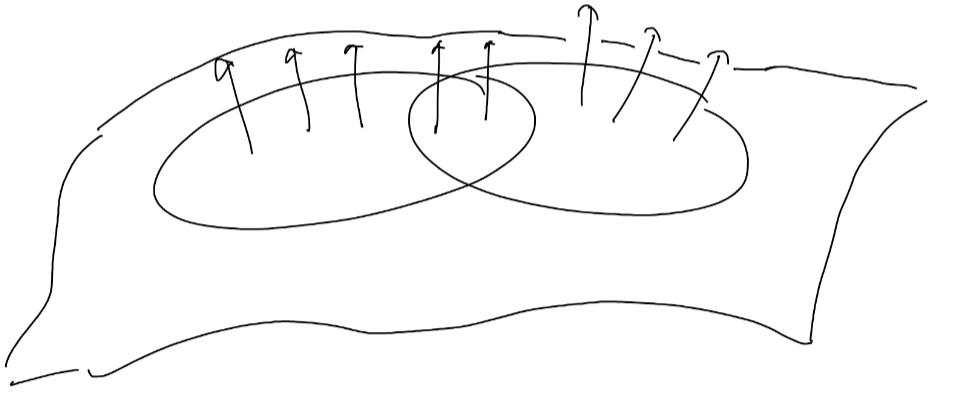
\includegraphics[width=0.5\linewidth]{orientierbare_untermannigfaltigkeit}
      \label{fig:orientierbare_untermannigfaltigkeit}
    \end{figure}
    Solche Parametrisierungen gibt es, da man durch Umsortieren der Komponentenfunktionen (\( * \)) erreichen kann.
  \end{proofdescription}
  
\end{proof}
      

\begin{beispiel*}
  \( \randpunkte G \) aus dem \hyperref[integralsatz_gauss]{Satz von Gauß} ist also orientierbar, das Möbiusband dagegen nicht (\( G \) ist ohnehin orientierbar).
\end{beispiel*}

\begin{bemerkung}
  Das Übertragen des Integrals über \( m \)-Formen auf \( m \)-dimensionale orientierbare Untermannigfaltigkeiten funktioniert wie zuvor:
  \begin{itemize}
      \item Zunächst für \( m=n \) (siehe oben)
      \item Dann für \( K\subset M\subset\reals^m \) (\( n\geq m \)).
      \( K \) kompakt unter der Annahme, dass 
      \begin{equation*}
          \exists \varphi\maps U\to \reals^n
      \end{equation*}
      mit \( K\subset \varphi(U) \). Mit \ref{pullback} folgt:
      \begin{equation*}
          \int_K \omega\coloneqq \int_{\varphi^{-1}(K)}\diffpullback{\varphi}{\omega}
      \end{equation*}
      ist eine sinnvolle Definition, die von der Wahl von \( \varphi \) nicht abhängt:
      \begin{equation*}
          \varphi=\psi\circ(\underbrace{\psi^{-1}\circ\varphi}_{\determinant{\totalderivative{\dotsb }}>0})
      \end{equation*}
      \item Dann für \( K\subset M \) mit \( \Set{\varphi_i\maps U_i\to V_i}_{i\in I} \) eine Beschreibung von \( M \) durch gleich orientierte Parametrisierungen.
      \( K \) kompakt \timplies endlich viele \( U_1,\dotsc ,U_l \) überdecken \( K \) \timplies Integralbegriff mit Hilfe einer untergeordneten Teilung der Eins.
  \end{itemize}
\end{bemerkung}

\begin{beispiel*}
  \( \omega=\p*{ \partial_1g-\partial_2f }\differential{x}\wedge\differential{y} \) auf \( U\subset \reals^2 \).
  Dann gilt für \( G\subset U \) wie im \hyperref[integralsatz_gauss]{Satz von Gauß} 
  \begin{equation*}
      \int_G\omega=\int_{\partial G}\scalarproduct{F}{\nu}\differential{s(t)}
  \end{equation*}
  mit \( F=\begin{psmallmatrix} g\\-f \end{psmallmatrix} \)
  \begin{figure}[H]
    \centering
    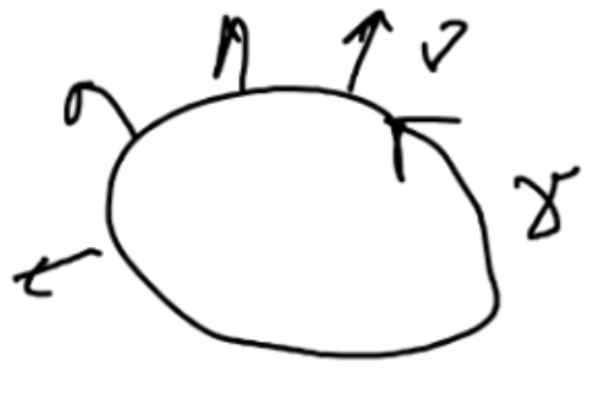
\includegraphics[width=0.3\linewidth]{stokes_motivation}
    \label{fig:stokes_motivation}
  \end{figure}
  \begin{equation*}
      \differential{s(t)}=\sqrt{\determinant{\totalderivative{\gamma}}}\differential{t}=\euclidiannorm{\gamma'(t)}\differential{t},\quad \nu(\gamma(t))=\begin{pmatrix} \gamma_2'(t)\\-\gamma_1'(t) \end{pmatrix} \frac{1}{\euclidiannorm{\gamma}} 
  \end{equation*}
  Also 
  \begin{align*}
      \int_{G}\omega &= \int_{\partial G}\scalarproduct{Fv}\differential{s(t)}\\
      &= \int_{a}^{b}\p*{ F_1\p*{\gamma(t)}\gamma_2'(t)-F_2\p*{\gamma(t)}\gamma_1'(t) }\differential{t}\\
      &\explain[Big]{ \differential{x^i}=\differential{\p*{ \gamma_i(t) }}=\gamma_i'\differential{t}}{=}
      \int_{\partial G}F_1\differential{y}-F_2\differential{x}\\
      &= \int_{\partial G}\underbrace{g\differential{y}+f\differential{x}}_{\eqqcolon \alpha}
  \end{align*}
  Notation aus \thref{satz_von_gauss}.
  Es ist \( \omega=\differential{\alpha}=\p*{ \partial_1g-\partial_2f }\differential{x}\wedge\differential{y} \).
  Also schreibt sich der Satz von Gauß hier:
  \begin{equation*}
      \int_{G}\differential{\alpha}=\int_{\partial G}\alpha
  \end{equation*}
  Das ist kein Zufall! (siehe unten)
\end{beispiel*}

Zunächst etwas Vorarbeit:

\begin{satz}
  Sei \( M \) orientierbare, \( m \)-dimensionale Mannigfaltigkeit in \( \reals^n \) mit Rand.
  Dann ist auch die \( (m-1) \)-dimensionale Untermannigfaltigkeit \( \partial M \) orientierbar.
\end{satz}

\begin{proof}[Beweis-Idee]
  Sei \( \varphi\maps U\to V \) Parametrisierung (\( U\subset \reals_{eq 0}\times \reals^{m-1} \) offen) \sd \( \varphi\p*{ U\cap\set{0}\times \reals^{m-1}=V\cap\partial M\neq \emptyset } \)
  \begin{figure}[H]
    \centering
    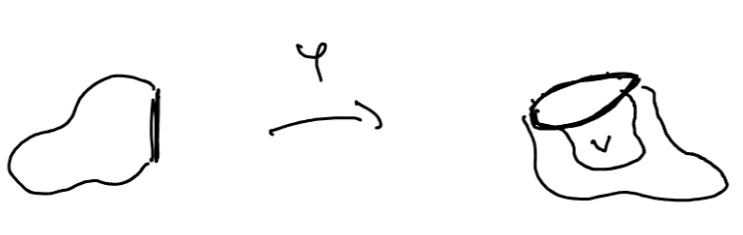
\includegraphics[width=0.5\linewidth]{randparametisierung}
    \label{fig:randparametisierung}
  \end{figure}
  und \( \set{\varphi,\varphi_i}_j \) sei eine Beschreibung von \( M \) durch orientierte Parametrisierung.

  Betrachte die letzte Spalte von \( \differential{\varphi} \), also 
  \begin{equation*}
      \totalderivative{\varphi}(t_0)\matrixmult e_m\eqqcolon v,\quad \varphi(t_0)=p\in\partial M
  \end{equation*}
  \begin{figure}[H]
    \centering
    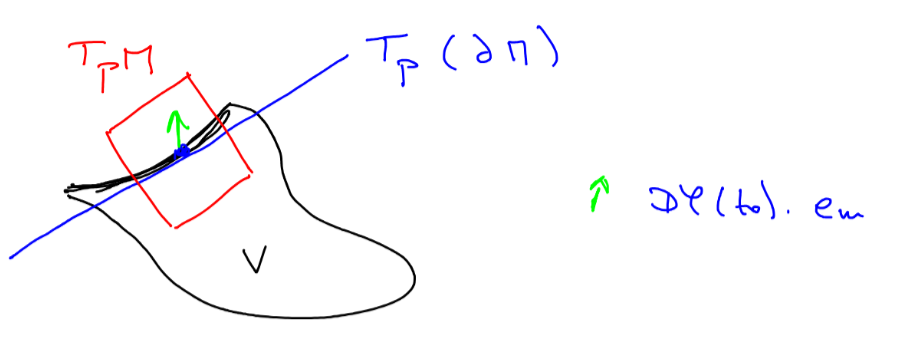
\includegraphics[width=0.5\linewidth]{tangentialraum_mannigfaltigkeit_und_rand}
    \label{fig:tangentialraum_mannigfaltigkeit_und_rand}
  \end{figure}
  Eine Basis \( (w_1,\dotsc ,w_{m-1}) \) von \( \tangentialraum{p}{\partial M} \) ist dann so zu wählen, dass die Basis \( (v,w_1,\dotsc ,w_{m-1}) \) von \( \tangentialraum{p}{M} \) gleich orientiert ist wie die Orientierung von \( \tangentialraum{p}{M}  \).
\end{proof}
\begin{bemerkung*}
  Mann nennt diese Orientierung als die von der Orientierung von \( M \) induzierte.
\end{bemerkung*}
\begin{beispiel*}\

  \( \overline{D} \) 
  \begin{figure}[H]
    \centering
    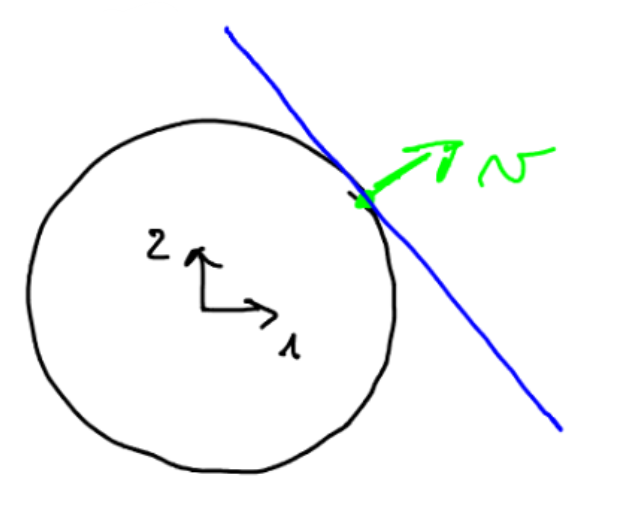
\includegraphics[width=0.5\linewidth]{disk_rand_orientierung}
    \label{fig:disk_rand_orientierung}
  \end{figure}
  \( (v,w) \) orientiert wie \( \reals^2 \) mit \( (e_1,e_2)\implies w\nwarrow \)

  \timplies Der Rand wird von den orientierten Parametrisierungen gegen Uhrzeigersinn durchlaufen.
\end{beispiel*}


\begin{satz}[Spezialfall des Satzes von Stokes]\index[theorems]{Spezialfall des Satzes von Stokes}
  \label{stokes_spezialfall}
  Sei \( \omega\in\differentialforms{m-1}{\reals^m} \) \( \stetigefunktionen[1] \) und mit kompaktem Träger \( \traeger{\omega} \)
  (\( \traeger{\omega}=\abschluss{\Set*{p\in\reals^m| \omega(p)\neq \text{Nullform}}} \) in Koordinaten: \( \omega_{i_1\cdots i_{m-1}} \) hat kompakte Träger).
  Dann gilt:
  \begin{equation*}
      \int_{\reals_-^m}\differential{\omega}=\int_{\partial\reals_-^m}\omega
  \end{equation*}
  wobei \( \reals_-^m=\reals_{eq 0}\times \reals^{m-1}\), \( \partial\reals_-^m=\set{0}\times \reals^{m-1} \).
\end{satz}

\begin{proof}
  \begin{align*}
      \omega &= \sum \omega_{i_1\cdots i_{m-1}}\differential{x^{i_1}}\wedge\dotsb \wedge\differential{x^{i_{m-1}}}\\
      &\eqqcolon \sum_{j=1}^{m}(-1)^{j-1}\alpha_j\differential{x^1}\wedge\dotsb \wedge \underset{\text{fehlt}}{\widehat{\differential{x^j}}}\wedge\dotsb\wedge\differential{x^n}
  \end{align*}
  Kompakter Träger \timplies \texists \( K \) kompakt \sd \( \evaluateat{\alpha_j}{\reals^m\setminus K}=0 \forall j \)
  \begin{gather*}
      \differential{\omega}=\sum_{j=1}^{m}\left( \partial_1\alpha_j \right)\differential{x^1}\wedge\dotsb \wedge\differential{x^m}\\
      \varphi\colon \reals^{m-1}\to \partial\reals_-^{m-1},\quad \left( t^1\dotsm t^{m-1} \right) \mapsto \left( 0,t^1,\dotsc ,t^{m-1} \right)\\
      \varphi^*\omega=\sum_{j=1}^{m}(-1)^{j-1}(\alpha_j\circ\varphi)\differential{\varphi^1}\wedge\dotsb \wedge\widehat{\differential{\varphi^j}}\wedge\dotsb \wedge\differential{\varphi^m}\\
      \differential{\varphi^1}=0\quad (\varphi^1(t)=0 \forall t)\\
      \differential{\varphi^j}=\differential{t^{j-1}}\quad (\varphi^j(t)=t^{j-1})\text{ für }j\geq 2\\
      \begin{aligned}[t]
          &\implies \varphi^*\omega=(\alpha_1\circ\varphi)\differential{t^1}\wedge \dotsb \wedge \differential{t}^{m-1}\\
          &\implies \int_{\partial\reals_-^m}\omega=\int_{\reals^{m-1}}\differential{\omega}=\int_{\reals^{m-1}}\alpha_1(0,t^1,\dotsc ,t^{m-1})\differential{t}
      \end{aligned}
  \end{gather*}
  Linke Seite:
  \begin{gather*}
      \int_{R_-^m}\differential{\omega}=\int_{\reals_-^m}\left( \sum_{j=1}^{m}\partial_j\alpha_j \right)\differential{x}\\
      \int_{\reals\leq 0}\partial_1\alpha_1(x)\differential{x^1}=\int_{-\infty}^{0}\partial_1\alpha_1(x)\differential{x^1}=\alpha_1(0,x^2,\dotsc ,x^m)\\
      \int_{\reals\leq 0\times \reals^{m-2}}\Bigg(
      \underbrace{\int_{-\infty}^{\infty}\partial_j\alpha_j(x)\differential{x_j}}_{=0}    
      \Bigg)\differential{x_1}\dotsb \widehat{\differential{x_j}}\dotsb \differential{x_m}
  \end{gather*}
  \timplies Beh.
\end{proof}

\begin{satz}[Integralsatz von Stokes] \index[theorems]{Integralsatz von Stokes}\label{integralsatz_stokes}
  Sei \( M \) orientierte \( m \)-dimensionale Untermannigfaltigkeit des \( \reals^n \) mit Rand \( \partial M \), der die induzierte Orientierung trägt.
  Sei \( \omega\in\differentialforms{m-1}{M} \) mit kompaktem Träger und \( \stetigefunktionen[1] \). Dann gilt 
  \begin{equation*}
      \int_M\differential{\omega}=\int_{\partial M}\omega.
  \end{equation*}
\end{satz}

\begin{proof}[Beweisidee]
  Sei \( \varphi\colon U\to M \) globale Parametisierung von \( \traeger{\omega} \) (sonst: Zerlegung der Eins).
  Setze \( \varphi^*\omega \) durch 0 fort zu einer Differentialform auf ganz \( \reals_-^m \).
  \begin{itemize}
      \item Ist \( U \) offen in \( \reals^m \) ist \( \varphi(U)\cap \partial M=\emptyset \). Beide Seiten sind 0.
      \item Ist \( U \) offen in \( \reals_-^m \) also \( \varphi(U)\cap \partial M\neq\emptyset \), gilt 
      \begin{align*}
          \int_M\differential{\omega} &= \int_U\varphi^*(\differential{\omega})\explain{\text{Nachrechnen!}}{=}\int_U\differential{(\varphi^*\omega)}\\
          &= \int_{\reals_-^m}\differential{(\varphi^*\omega)} \overset{\text{\ref{stokes_spezialfall}}}{=}\int_{\partial\reals_-^m}\varphi^*\omega\\
          &= \int_{\partial U}\varphi^*\omega\explain{\evaluateat{\varphi}{\partial U}}{=}\int_{\varphi(\partial M)}\omega=\int_{\partial M}\omega
      \end{align*}
  \end{itemize}
\end{proof}

\begin{beispiel*}
  \hyperref[integralsatz_gauss]{Satz von Gauß},\dots.
\end{beispiel*}

\begin{beispiel*}
  \( n=3\quad \omega=f_1\differential{x^1}+f_2\differential{x^2}+f_3\differential{x^3} \)
  \begin{align*}
      \differential{\omega}&= \left( \partial_2f_3-\partial_3f_2 \right)\differential{x^2}\wedge \differential{x^3}\\
      &+\left( \partial_3f_1-\partial_1f_3 \right) \differential{x^3}\wedge \differential{x^1}\\
      &+\left( \partial_1f_2-\partial_2f_1 \right)\differential{x^1}\wedge \differential{x^2}
  \end{align*}
  Koeffizienten heißen auch Rotation von \( f=\begin{psmallmatrix} f_1\\f_2\\f_3 \end{psmallmatrix} \)
  \begin{figure}[H]
    \centering
    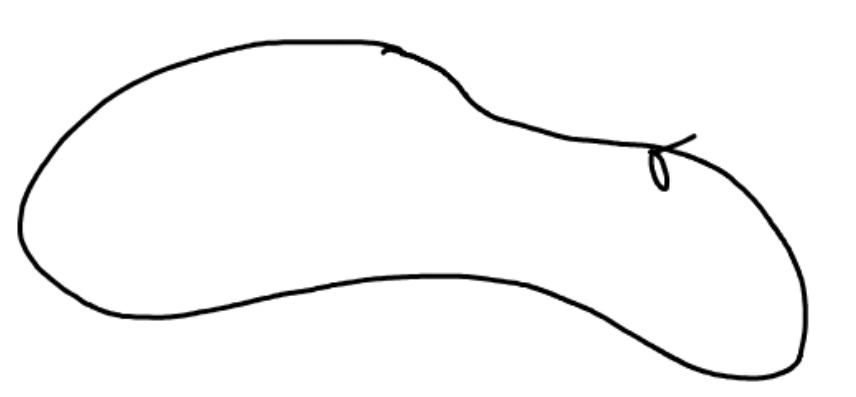
\includegraphics[width=0.5\linewidth]{stokes_beispiel}
    \label{fig:stokes_beispiel}
  \end{figure}
  \begin{equation*}
      M\quad \text{2-dim }\subset \reals^3
  \end{equation*}
  \begin{equation*}
      \int_M\differential{\omega}=\int_{\partial M}\omega\quad \text{Kurvenintegral \vgl Beispiel nach \ref{uebertragung_integral}}
  \end{equation*}
  \begin{align*}
      \int f_1\differential{x^1}+\dotsb +f_3\differential{x^3} &= \int\left( f_1\left( \gamma(t) \right)\gamma_1'(t)+\dotsb +f_3\left( \gamma(t) \right)\gamma_3'(t) \right)\differential{t}\\
      &= \int\scalarproduct{f(\gamma(t)}{\gamma'(t))}\differential{t}
  \end{align*}
\end{beispiel*}

